% Options for packages loaded elsewhere
\PassOptionsToPackage{unicode}{hyperref}
\PassOptionsToPackage{hyphens}{url}
\PassOptionsToPackage{dvipsnames,svgnames,x11names}{xcolor}
%
\documentclass[
  letterpaper,
  DIV=11,
  numbers=noendperiod]{scrartcl}

\usepackage{amsmath,amssymb}
\usepackage{iftex}
\ifPDFTeX
  \usepackage[T1]{fontenc}
  \usepackage[utf8]{inputenc}
  \usepackage{textcomp} % provide euro and other symbols
\else % if luatex or xetex
  \usepackage{unicode-math}
  \defaultfontfeatures{Scale=MatchLowercase}
  \defaultfontfeatures[\rmfamily]{Ligatures=TeX,Scale=1}
\fi
\usepackage{lmodern}
\ifPDFTeX\else  
    % xetex/luatex font selection
\fi
% Use upquote if available, for straight quotes in verbatim environments
\IfFileExists{upquote.sty}{\usepackage{upquote}}{}
\IfFileExists{microtype.sty}{% use microtype if available
  \usepackage[]{microtype}
  \UseMicrotypeSet[protrusion]{basicmath} % disable protrusion for tt fonts
}{}
\makeatletter
\@ifundefined{KOMAClassName}{% if non-KOMA class
  \IfFileExists{parskip.sty}{%
    \usepackage{parskip}
  }{% else
    \setlength{\parindent}{0pt}
    \setlength{\parskip}{6pt plus 2pt minus 1pt}}
}{% if KOMA class
  \KOMAoptions{parskip=half}}
\makeatother
\usepackage{xcolor}
\setlength{\emergencystretch}{3em} % prevent overfull lines
\setcounter{secnumdepth}{5}
% Make \paragraph and \subparagraph free-standing
\makeatletter
\ifx\paragraph\undefined\else
  \let\oldparagraph\paragraph
  \renewcommand{\paragraph}{
    \@ifstar
      \xxxParagraphStar
      \xxxParagraphNoStar
  }
  \newcommand{\xxxParagraphStar}[1]{\oldparagraph*{#1}\mbox{}}
  \newcommand{\xxxParagraphNoStar}[1]{\oldparagraph{#1}\mbox{}}
\fi
\ifx\subparagraph\undefined\else
  \let\oldsubparagraph\subparagraph
  \renewcommand{\subparagraph}{
    \@ifstar
      \xxxSubParagraphStar
      \xxxSubParagraphNoStar
  }
  \newcommand{\xxxSubParagraphStar}[1]{\oldsubparagraph*{#1}\mbox{}}
  \newcommand{\xxxSubParagraphNoStar}[1]{\oldsubparagraph{#1}\mbox{}}
\fi
\makeatother


\providecommand{\tightlist}{%
  \setlength{\itemsep}{0pt}\setlength{\parskip}{0pt}}\usepackage{longtable,booktabs,array}
\usepackage{calc} % for calculating minipage widths
% Correct order of tables after \paragraph or \subparagraph
\usepackage{etoolbox}
\makeatletter
\patchcmd\longtable{\par}{\if@noskipsec\mbox{}\fi\par}{}{}
\makeatother
% Allow footnotes in longtable head/foot
\IfFileExists{footnotehyper.sty}{\usepackage{footnotehyper}}{\usepackage{footnote}}
\makesavenoteenv{longtable}
\usepackage{graphicx}
\makeatletter
\def\maxwidth{\ifdim\Gin@nat@width>\linewidth\linewidth\else\Gin@nat@width\fi}
\def\maxheight{\ifdim\Gin@nat@height>\textheight\textheight\else\Gin@nat@height\fi}
\makeatother
% Scale images if necessary, so that they will not overflow the page
% margins by default, and it is still possible to overwrite the defaults
% using explicit options in \includegraphics[width, height, ...]{}
\setkeys{Gin}{width=\maxwidth,height=\maxheight,keepaspectratio}
% Set default figure placement to htbp
\makeatletter
\def\fps@figure{htbp}
\makeatother

\KOMAoption{captions}{tableheading,figureheading}
\makeatletter
\@ifpackageloaded{caption}{}{\usepackage{caption}}
\AtBeginDocument{%
\ifdefined\contentsname
  \renewcommand*\contentsname{Table of contents}
\else
  \newcommand\contentsname{Table of contents}
\fi
\ifdefined\listfigurename
  \renewcommand*\listfigurename{List of Figures}
\else
  \newcommand\listfigurename{List of Figures}
\fi
\ifdefined\listtablename
  \renewcommand*\listtablename{List of Tables}
\else
  \newcommand\listtablename{List of Tables}
\fi
\ifdefined\figurename
  \renewcommand*\figurename{Figure}
\else
  \newcommand\figurename{Figure}
\fi
\ifdefined\tablename
  \renewcommand*\tablename{Table}
\else
  \newcommand\tablename{Table}
\fi
}
\@ifpackageloaded{float}{}{\usepackage{float}}
\floatstyle{ruled}
\@ifundefined{c@chapter}{\newfloat{codelisting}{h}{lop}}{\newfloat{codelisting}{h}{lop}[chapter]}
\floatname{codelisting}{Listing}
\newcommand*\listoflistings{\listof{codelisting}{List of Listings}}
\makeatother
\makeatletter
\makeatother
\makeatletter
\@ifpackageloaded{caption}{}{\usepackage{caption}}
\@ifpackageloaded{subcaption}{}{\usepackage{subcaption}}
\makeatother

\ifLuaTeX
  \usepackage{selnolig}  % disable illegal ligatures
\fi
\usepackage{bookmark}

\IfFileExists{xurl.sty}{\usepackage{xurl}}{} % add URL line breaks if available
\urlstyle{same} % disable monospaced font for URLs
\hypersetup{
  pdftitle={STA107 Post-Course Survey Analysis},
  pdfauthor={Sinan Ma; Jaiditya Dev},
  colorlinks=true,
  linkcolor={blue},
  filecolor={Maroon},
  citecolor={Blue},
  urlcolor={Blue},
  pdfcreator={LaTeX via pandoc}}


\title{STA107 Post-Course Survey Analysis}
\usepackage{etoolbox}
\makeatletter
\providecommand{\subtitle}[1]{% add subtitle to \maketitle
  \apptocmd{\@title}{\par {\large #1 \par}}{}{}
}
\makeatother
\subtitle{Evaluating Student Reflections on R and Statistical Learning}
\author{Sinan Ma \and Jaiditya Dev}
\date{2025-04-13}

\begin{document}
\maketitle

\renewcommand*\contentsname{Table of contents}
{
\hypersetup{linkcolor=}
\setcounter{tocdepth}{3}
\tableofcontents
}

\section{Introduction}\label{introduction}

This report presents an analysis of the anonymous post-course survey
completed by students enrolled in \textbf{STA107: Introduction to
Statistics} at the University of Toronto Mississauga. The survey was
voluntary, open for multiple submissions, and contributed \textbf{2\% to
the course grade}. Its goal was to evaluate students' experiences with
R-based activities, the integration of normal distribution concepts, and
overall satisfaction with the course components. This feedback will help
refine future course offerings and improve the learning experience.

\section{Survey Questions}\label{survey-questions}

This section outlines the structure of the survey and highlights key
question types:

\begin{itemize}
\tightlist
\item
  \textbf{Quantitative items}: Likert-scale responses on course clarity,
  usefulness of R exercises, and understanding of statistical concepts.
\item
  \textbf{Qualitative items}: Open-ended prompts for students to share
  what they found most/least helpful and suggestions for improvement.
\end{itemize}

The post-course survey comprised 17 open- and close-ended questions.
Among these, 8 were qualitative in nature (\texttt{Q3}, \texttt{Q6},
\texttt{Q8}, \texttt{Q10}, \texttt{Q11}, \texttt{Q12}, \texttt{Q13},
\texttt{Q14}, \texttt{Q15}, \texttt{Q16}, \texttt{Q17}), focusing on
free-text responses reflecting students' thoughts on the content,
instruction, and overall experience.

\section{Data Analysis}\label{data-analysis}

\subsection{Methodology}\label{methodology}

We employed a \textbf{mixed-methods approach}:

\begin{itemize}
\tightlist
\item
  \textbf{Quantitative analysis}: Descriptive statistics and
  visualizations for Likert-scale questions.
\item
  \textbf{Qualitative analysis}: Thematic coding of open-ended responses
  to identify common sentiments and suggestions.
\end{itemize}

\subsection{Quantitative Analysis}\label{quantitative-analysis}

\subsubsection{Communication Ability Before
vs.~After}\label{communication-ability-before-vs.-after}

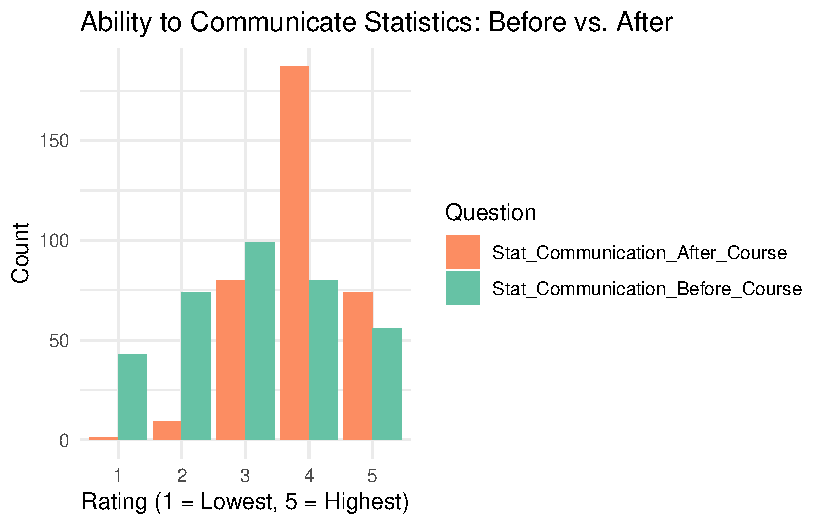
\includegraphics{paper_files/figure-pdf/unnamed-chunk-3-1.pdf}

The histogram shows a clear improvement in students' perceived
communication ability. More students rated themselves at level 4 or 5
after the course compared to before, indicating that the course helped
them gain confidence in articulating statistical ideas.

\subsubsection{R Ability Before
vs.~After}\label{r-ability-before-vs.-after}

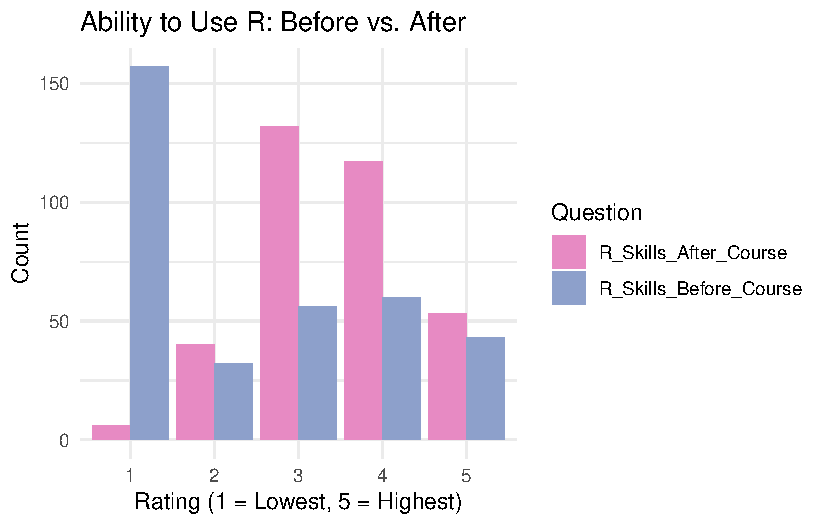
\includegraphics{paper_files/figure-pdf/unnamed-chunk-4-1.pdf}

Students entered the course with relatively low self-reported R skills
(mostly 1s and 2s), but after completing the course, a majority rated
themselves at 3 or higher. This shift demonstrates the course's success
in introducing R programming effectively.

\subsubsection{Understanding After Assignments
vs.~Tutorials}\label{understanding-after-assignments-vs.-tutorials}

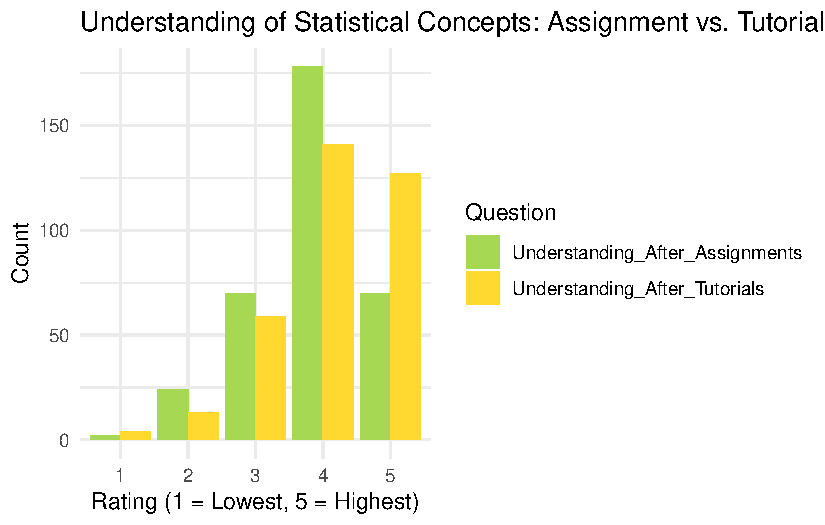
\includegraphics{paper_files/figure-pdf/unnamed-chunk-5-1.pdf}

Students found both tutorials and assignments useful for understanding
statistical concepts, with a slight preference for tutorials. The higher
number of level 4 and 5 responses for tutorials suggests that real-time,
interactive support may have been especially beneficial.

\subsection{Qualitative Analysis}\label{qualitative-analysis}

\section{Results}\label{results}

\subsection{Quantitative Results}\label{quantitative-results}

The survey included six Likert-scale questions aimed at capturing
students' self-perceived development in statistical understanding and
communication, both before and after the course. The questions also
addressed students' ability to use R software and their comprehension of
statistical concepts through tutorials and weekly assignments.

Key findings include:

\begin{itemize}
\tightlist
\item
  \textbf{Improved Communication Skills}: Students reported a notable
  improvement in their ability to communicate statistics, with the
  average post-course rating (M = 3.92) higher than the pre-course
  rating (M = 3.09).
\item
  \textbf{Increased R Proficiency}: The mean rating for R software usage
  rose from 2.43 before the course to 3.49 after completing it,
  indicating significant growth in computational skills.
\item
  \textbf{Conceptual Understanding}: Understanding of statistical
  concepts improved through both tutorials (M = 4.09) and weekly
  assignments (M = 3.84), with tutorials being rated slightly more
  helpful on average.
\end{itemize}

The graphs above illustrate the distribution of responses across the
three themes: communication, R proficiency, and statistical
understanding.

\subsection{Qualitative Results}\label{qualitative-results}

To gain deeper insights into student opinions, the qualitative analysis
comprised two parts: thematic analysis and sentiment analysis.

\subsubsection{Thematic Analysis}\label{thematic-analysis}

Following Braun and Clarke's (2006) framework, a sample of approximately
80 student responses was examined through six phases:

\begin{enumerate}
\def\labelenumi{\arabic{enumi}.}
\item
  \textbf{Familiarization}: Students' responses across 8 open-ended
  questions were read and annotated to gain an overall understanding.
\item
  \textbf{Generating Initial Codes}: Semantic-level codes were created
  to capture features related to course experience, R skill development,
  and content relevance.
\item
  \textbf{Searching for Themes}: Related codes were clustered into
  preliminary themes reflecting student attitudes and feedback.
\item
  \textbf{Reviewing Themes}: Themes were refined to ensure clarity and
  distinctiveness across the dataset.
\item
  \textbf{Defining and Naming Themes}: Clear definitions were
  established for each theme based on recurring patterns.
\item
  \textbf{Producing the Report}: Final themes were reported below with
  supporting quotes.
\end{enumerate}

\subsubsection{Identified Themes}\label{identified-themes}

\paragraph{Relevance to Real Life and
Careers}\label{relevance-to-real-life-and-careers}

Many students expressed appreciation for statistics content when it
connected to real-world examples or their field of study.

\begin{quote}
``This course gave me a solid foundation in statistical concepts and
taught me how to apply them using R. Overall, I gained practical skills
and became more confident in working with data.''
\end{quote}

\begin{quote}
``The course showed me how statistics applies to real-world problems,
such as data analysis in my ENV course as it has alot of data.''
\end{quote}

\paragraph{R as a Learning Tool}\label{r-as-a-learning-tool}

Students had mixed responses about learning R. While some found it
helpful, others found it initially intimidating.

\begin{quote}
``After the course, I had a higher opinion of my ability to use R
because I learned how to create visualizations and perform statistical
analyses such as normal distribution applications and regression. Now I
can use it to organize data, generate graphs, and interpret the output.
The tutorial session and assignments were particularly helpful in
helping me gradually build my skills.''
\end{quote}

\begin{quote}
``I have never worked with R, but after trying to work with it I
realized that it is also a powerful language.''
\end{quote}

\paragraph{Clarity and Structure of
Assignments}\label{clarity-and-structure-of-assignments}

Clearer instructions and expectations were a recurring theme.

\begin{quote}
``The weekly assignment was a R assignment based on the module. It was
sometimes hard to understand the purpose of the task.''
\end{quote}

\begin{quote}
``After completing the weekly assignments, I have a general
understanding of the statistical concepts in each module, but sometimes
I still have some difficulties understanding some difficult concepts.''
\end{quote}

\paragraph{Appreciation for Tutorials and TA
Support}\label{appreciation-for-tutorials-and-ta-support}

Tutorials and TA help sessions were viewed positively, especially for R
and concept reinforcement.

\begin{quote}
``For each question on the tutorial worksheet, my TA explained the
relevant concepts before attempting the problem, which helped me
understand the concept better. In addition, all tutorial exercises were
related to the weekly assignment, so it gave me reassurance that I was
doing everything correctly before submitting my assignments.''
\end{quote}

\begin{quote}
``The weekly tutorial was extremely useful for me. The worksheets were
helpful and my TA, Dylan, did an excellent job at explaining the
concepts involved and answering our questions when we were confused.''
\end{quote}

\begin{quote}
``my ta was great at explaining concepts and let us ask many questions
which would all get responses. very good by jaiditya.''
\end{quote}

\paragraph{Feedback and Reflection}\label{feedback-and-reflection}

Students wanted more timely or individualized feedback.

\begin{quote}
``I always read the feedback give by the TA's since they allowed me to
understand how to communicate my answers better. The statistical
examples did help me recognize the usefulness and value of learning
about statistics because it made me realize that statistics is
everywhere.''
\end{quote}

\begin{quote}
``Most of the feedback I recieved was in the form of checks or X. I feel
like I could have gotten a little bit better feedback but most of the
assignments I did were correct.''
\end{quote}

\subsubsection{Sentiment Analysis}\label{sentiment-analysis}

The sentiment analysis provided a quantitative measure of student
engagement across the survey's open-ended responses. Using the NRC
sentiment lexicon (implemented via the syuzhet package), we quantified
positive, negative, and neutral sentiments for each question.

The analysis revealed:

\begin{itemize}
\item
  \textbf{Predominantly Positive Sentiment}: Most responses expressed
  positive sentiments, especially regarding structured content delivery,
  effective use of R, and clear statistical explanations.
\item
  \textbf{Mixed Feedback on Clarity and Pace}: While many responses were
  positive overall, some negative sentiments were associated with
  challenges such as rapid topic progression and difficulties with R
  syntax.
\item
  \textbf{Critical Comments}: Negative terms like ``confusing,''
  ``fast,'' and ``examples'' frequently appeared in responses about
  areas needing clearer instructional support.
\end{itemize}

The bar chart above (generated in the sentiment analysis code chunk)
illustrates the distribution of sentiment (positive, negative, neutral)
for each of the 8 survey questions.

\begin{figure}[H]

\caption{Sentiment Distribution by Survey Question}

{\centering 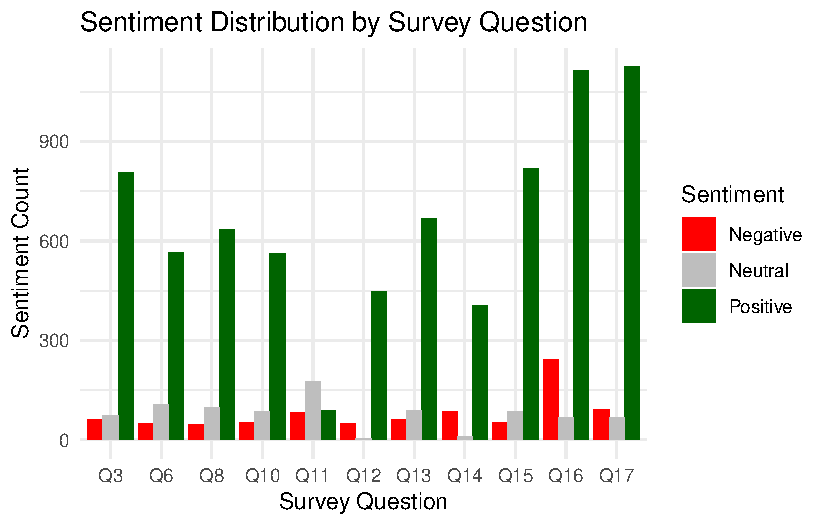
\includegraphics{paper_files/figure-pdf/sentiment-plot-1.pdf}

}

\end{figure}%

\section{Conclusion}\label{conclusion}

The STA107 post-course survey provides valuable insights into how
students perceive the course structure and its technical components.
Findings highlight both effective practices and opportunities for
enhancement. Continued evaluation and iteration will ensure the course
remains responsive to student needs and pedagogical best practices.

From a qualitative perspective, student feedback revealed strong
appreciation for several key elements of the course especially the
hands-on R activities, the integration of real-world statistical
examples, and the clarity of normal model explanations. These components
were described as engaging and instructive, affirming their value in
helping students apply theoretical knowledge in practical settings.

However, when students were asked about areas of improvement, many
raised concerns regarding the speed at which complex topics were
introduced, as well as the difficulty of interpreting R-based
assignments without more structured guidance. Themes of pacing, clarity,
and the need for more scaffolded instruction were particularly
prominent. Addressing these concerns by slowing down the delivery of
technical material, providing more detailed examples, and incorporating
mid-semester feedback opportunities could significantly enhance the
learning experience in future offerings of STA107.

\section{References}\label{references}

\begin{itemize}
\item
  Jockers, M. (2017). \emph{syuzhet: Extracts Sentiment and
  Sentiment-Derived Plot Arcs from Text} (R package v1.0.4).
  \href{https://cran.r-project.org/web/packages/syuzhet/index.html}{CRAN
  Documentation}
\item
  Jockers, M. (2020). \emph{Introduction to the Syuzhet Package}.
  \href{https://cran.r-project.org/web/packages/syuzhet/vignettes/syuzhet-vignette.html}{CRAN
  Vignette}
\item
  Kim, H. (2022). Sentiment Analysis: Limits and Progress of the Syuzhet
  Package and Its Lexicons. \emph{Digital Humanities Quarterly, 16}(2).
  \href{http://www.digitalhumanities.org/dhq/vol/16/2/000601/000601.html}{Article}
\end{itemize}




\end{document}
